\chapter{Definitionen}
\label{cha:Definitionen}

\section{Bring Your Own Device}
In der heutigen Arbeitswelt hat die Geschwindigkeit ein Produkt auf den Markt zu bringen so sehr an Wert gewonnen, damit man dem ständigen Wettbewerb gerecht wird und somit als Unternehmen überlebt. Hierbei ist es nicht nur wichtig schnell zu sein, sondern auch flexibel. Dazu gehört in einem Unternehmen, die Möglichkeit, wo- und wann auch immer, Arbeit zu verrichten, zu den Voraussetzungen und Treibern Erfolg im Wettkampf mit der Konkurrenz zu haben. Die Denkweise der Arbeitnehmer heutiger Zeit, hat sich durch Globalisierung und Vernetzung so angepasst, dass es darum geht, welche Arbeit getan werden muss, und nicht wo. Der Arbeitsplatz soll nicht mehr auf das Büro beschränkt sein. Ein Arbeiten von zuhause und unterwegs, ist wegen der ständigen Bewegung in der "Online"-Welt, wichtiger denn je. Die Grenze zwischen Arbeit und Leben der Arbeitnehmer vermischt sich immer mehr.

Bring Your Own Device (BYOD) beschreibt eine IT-Richtlinie, die, wie die deutsche Übersetzung "Bring dein eigenes Gerät", offenbart, Mitarbeitern eines Unternehmens erlaubt, eigene private Geräte im geschäftlichen Umfeld zu nutzen. Zu den Geräten dieser "Trend"-Richtlinie gehören hauptsächlich die Nutzung von Smartphones, aber auch Tablets oder Laptops sind denkbar umsetzbar. Um BYOD umsetzen zu können, werden EMM-Plattformen eingesetzt, welche die Trennung einer Arbeits- und Privatwelt auf den Geräten ermöglicht und dabei die Sicherheitsrichtlinien des Unternehmens einhält. Bevor jedoch erklärt wird, wie BYOD Lösungen umgesetzt werden können, gilt zuerst die Frage zu beantworten warum es zu dieser IT-Bewegung kommt.

\subsection{Vorteile}
In einer Studie von Extreme Networks \cite{ext2014} wurden deutsche Unternehmen nach Vorteilen, die sie sich aus dem Nutzen von BYOD erhoffen. Als Ergebnis, siehe \cref{fig:VorBYOD} sind 43\% erhöhte Mitarbeiterzufriedenheit, 32\% erhöhte Produktivität der Mitarbeiter, 16\% Kosteneinsparungen und 9\% andere Gründe zu vermerken.
\begin{figure}[hbt]
\centering
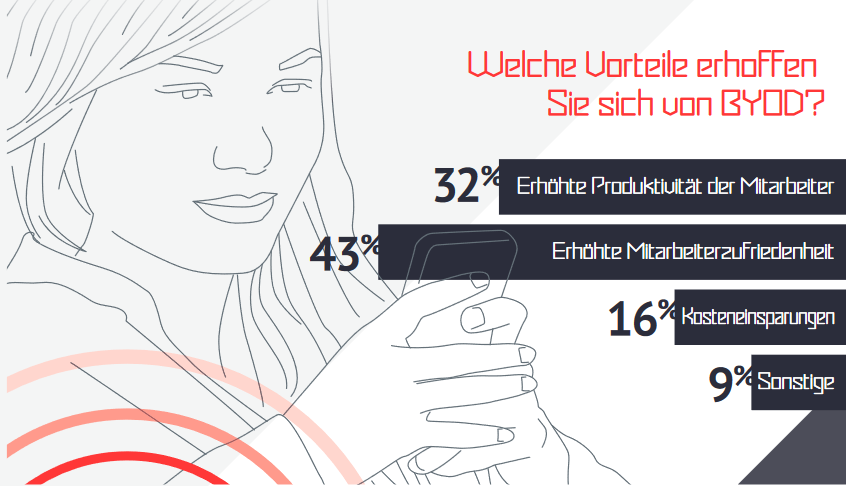
\includegraphics[width=0.95\textwidth]{Bilder/Vorteile_BYOD.png} 
\caption{Umfrage: Erhoffte Vorteile von BYOD}\label{fig:VorBYOD}
\end{figure}
Diese Vorteile lassen sich in Vorteile für den Endnutzer und für das Unternehmen unterteilen.\footnote{Vgl. \cite{fuj2018} } Dem Endnutzer bietet die Umsetzung von BYOD den Vorteil, die Freiheit, das Gerät nach ihren Präferenzen auszuwählen. Wie oben beschrieben löst BYOD das Problem der Stationärität des Arbeitnehmers. Das Arbeiten von zuhause und unterwegs ist damit kein Problem mehr. Subjektiv ist, ob BYOD einen positiven Einfluss auf das Work-Life-Balance hat, aber es hat zumindest den Vorteil, dass die Integration von Leben und Arbeit möglich ist. Daraus erhoffen sich die Unternehmen, dass durch das Nutzen eines Gerätes für das private Leben sowie für die Arbeit, die Mitarbeiterzufriedenheit und gleichzeitig das Engagement steigt.

Es ist zu erkennen, dass nicht nur dem Endnutzer aus diesem Aspekt, ein Vorteil geboten ist. BYOD, daraus abgeleitet Mitarbeiterzufriedenheit, hat als weitere Folge, die Attraktivität und das Image eines Unternehmens aufzubessern und so weitere qualifizierte Mitarbeiter zu gewinnen. Denn als Ziel von Unternehmen gilt wie in traditionellerweise die Suche von Talenten. Der Technologiefortschritt und die Flexibilität eines Arbeitsplatzes ist im Vergleich zum konventionellen Angebot eines Firmenwagens mittlerweile deutlich attraktiver und erhält immer größere Signifikanz. 

Das Mitarbeiter, ihre Arbeit mit dem Privatleben vermischen, bringt Unternehmen weitere Vorteile. Es ist Möglich zusätzlich neben den normalen Arbeitszeiten an Wochenenden zu arbeiten. Dies fördert nicht nur die komplette Produktivität sondern auch die Empfänglichkeit gegenüber der Kunden, welches weiterhin zu erhöhter Kundenzufriedenheit führt. Weiterhin verringert sich dadurch die Antwortzeit auf den Markt, fördert Innovation und sichert damit einen Vorsprung im Wettbewerb.

Wie in der Umfrage beschrieben, erhoffen sich Unternehmen einen Vorteil durch Kosteneinsparungen durch die Einführung von BYOD. Die Frage ob durch die Umsetzung ein Kostenvorteil entsteht und ist nicht direkt ablesbar, da es komplett abhängig von der vorher genutzten Infrastruktur eines Unternehmens ist. Nimmt man ein Unternehmen, welches viel Geld in Firmengelände investiert, damit dort die Mitarbeiter arbeiten können, ist ein großer Kostenvorteil denkbar. Denn lässt dieses mithilfe von BYOD einen Großteil der Mitarbeiter von zuhause arbeiten, können Ausgaben für Gelände und Arbeitsorte gespart werden. 
Da Nutzer ihr eigenes Gerät verwenden, steigt die Fürsorge und Vorsicht darum. So können Kosten für Wartung und Ersatzvergabe präventiv klein gehalten werden.










\section{Mobile Device Management (MDM)}
Mobile Device Management (MDM) ist eine Technologie zur Lebenszyklusverwaltung, mit der die IT Mobilgeräte durch auf den Geräten installierte MDM-Profile einsetzen, konfigurieren, verwalten, unterstützen und sichern kann. MDM Software ermöglicht Anlageninventur, Over-the-Air-Konfiguration von E-Mail, Anwendungen und WLAN, Remotefehlerbehebung sowie Remotesperr- und Remote Wipe-Funktionen zur Sicherung von Geräten und den darauf befindlichen Unternehmensdaten. MDM ist die Grundlage für eine umfassende Enterprise Mobility Management-Lösung (EMM). 

\section{Mobile Application Management}
Mobile Application Management-Technologien (MAM) wenden Tools der Verwaltungs- und Richtlinienkontrolle auf individuelle Anwendungen statt auf das gesamte Gerät an. Üblicherweise bieten MAM-Lösungen einen benutzerdefinierten App Store, der die Kontrolle und Bereitstellung von sowohl intern entwickelten als auch Drittanbieteranwendungen erlaubt. IT-Administratoren haben die Möglichkeit, mithilfe von AppConfig Community-Standards oder Software Development Kit- oder App Wrapping-Lösungen vom MAM-Anbieter der Anwendung Sicherheits-, Verschlüsselungs- und Kontrollfunktionen hinzuzufügen. 

\section{Mobile Content Management}

\section{Enterprise Mobility Management}
Enterprise Mobility Management (EMM) ist eine geräte- und plattformagnostische Lösung, in der die Verwaltung, Konfiguration und Sicherheit aller Geräte – BYO sowie unternehmenseigenen – einer Organisation zusammengefasst werden. EMM erstreckt sich über traditionelle Geräteverwaltung hinaus auf die Verwaltung und Konfiguration von Unternehmensanwendungen und -inhalten.  Eine solide EMM-Lösung umfasst üblicherweise MDM, MAM, Mobile Content Management (MCM), Identitätsmanagement zur Zugriffskontrolle sowie Produktivitätsanwendungen zum mühelosen Zugriff auf E-Mail, Kalender, Kontakte, Inhalts-Repositorys und Intranet-Sites des Unternehmens. Darüber hinaus sollte eine EMM-Lösung es technisch ermöglichen, der IT die Verwaltung und Sicherheit zu erleichtern und gleichzeitig den Mitarbeitern ein angenehmes Benutzererlebnis zu bieten. 

\section{Unified Endpoint Management}
Mithilfe von Unified Endpoint Management (UEM) ist die IT endlich in der Lage, sich der unterschiedlichen Tools für die Verwaltung von Mobilgeräten, Desktops und seit Kurzem auch IdD-Geräten (Internet der Dinge) zu entledigen. Durch die Kombination von traditioneller Client-Verwaltung von Desktop- und PC-Systemen mit einem modernen Enterprise Mobility Management Framework (EMM) schaffen UEM-Lösungen die Voraussetzung für einen ganzheitlichen und anwenderorientierten Ansatz zur Verwaltung aller Endpunkte. Eine solide UEM-Lösung befähigt die IT zur Verwaltung von Benutzern und zur Realisierung eines einheitlichen Erlebnisses entlang aller Endpunkte sowie zur Sicherung und Verwaltung des gesamten Gerätelebenszyklus – und alles über eine zentrale, umfassende Plattform. 






